\chapter{Background}
\label{chap:background}

\ifpdf
	\graphicspath{{Chapter1/Chapter1Figs/PDF/}{Chapter1/Chapter1Figs/PNG/}
		{Chapter1/Chapter1Figs/}}
\else
	\graphicspath{{Chapter1/Chapter1Figs/EPS/}{Chapter1/Chapter1Figs/}}
\fi

There have been work going on to open Blue Gene for more generic applications,
and Plan 9 has been ported to Blue Gene\cite{Van07} as part of that effort.
This has lead to exploration of alternatives for workload distribution on this
platform.

Following are the concepts/work that inspired our exploration.  We have borrowed
many concepts from these works and used them to meet the requirements of dataflow applications.


\section{Plan 9}
Plan 9 is a distributed operating system which is able to simplify development of
distributed applications. The Plan 9 design is based on three primary design principles.
\begin{enumerate}
	\item \textbf{Everything is file} : Plan 9 presents everything as file. This includes
devices and the processor itself.  All these resources are accessible in a hierarchical
namespace.
	\item \textbf{9P: Standard communication protocol} All files are accessed using the
9P protocol. This allows accessing both local and remote resources in same way.
	\item \textbf{Namespaces} Each process has it's own namespace view.  This namespace
view can be separately built for every process, allowing every process to have
a different view of the world.\cite{namespace}
\end{enumerate}

As everything in Plan 9 is a file, it is easy to share everything as file over network.  It also
allows transparently sharing its resources as files over network.  The 9P protocol
removes the differentiation between local and remote resources by providing the same
interface for accessing both of them.  Private namespaces allow a process to build
its own namespace using any resources anywhere over the network.  These features allow
arranging any remote resources in any view and using them transparently.  In the following
sections, we will see how these concepts can be used to simplify the deployment
of applications on remote nodes.


\subsection{CPU}
CPU\cite{plan9-cpu} is Plan 9's concept for using remote compute resources.  It is 
different from traditional rlogin, telnet or ssh.  Most of these protocols work 
by logging in on a remote node and providing the environment of the remote node to user.
Only the local terminal is used while all other resources like the processor, disk and 
filesystem are from the remote node.

In contrast, CPU works by bringing remote resources to the user.  Figure 2.1 presents
CPU.
\begin{figure}[h]
  \begin{center}
    \leavevmode
    \ifpdf
      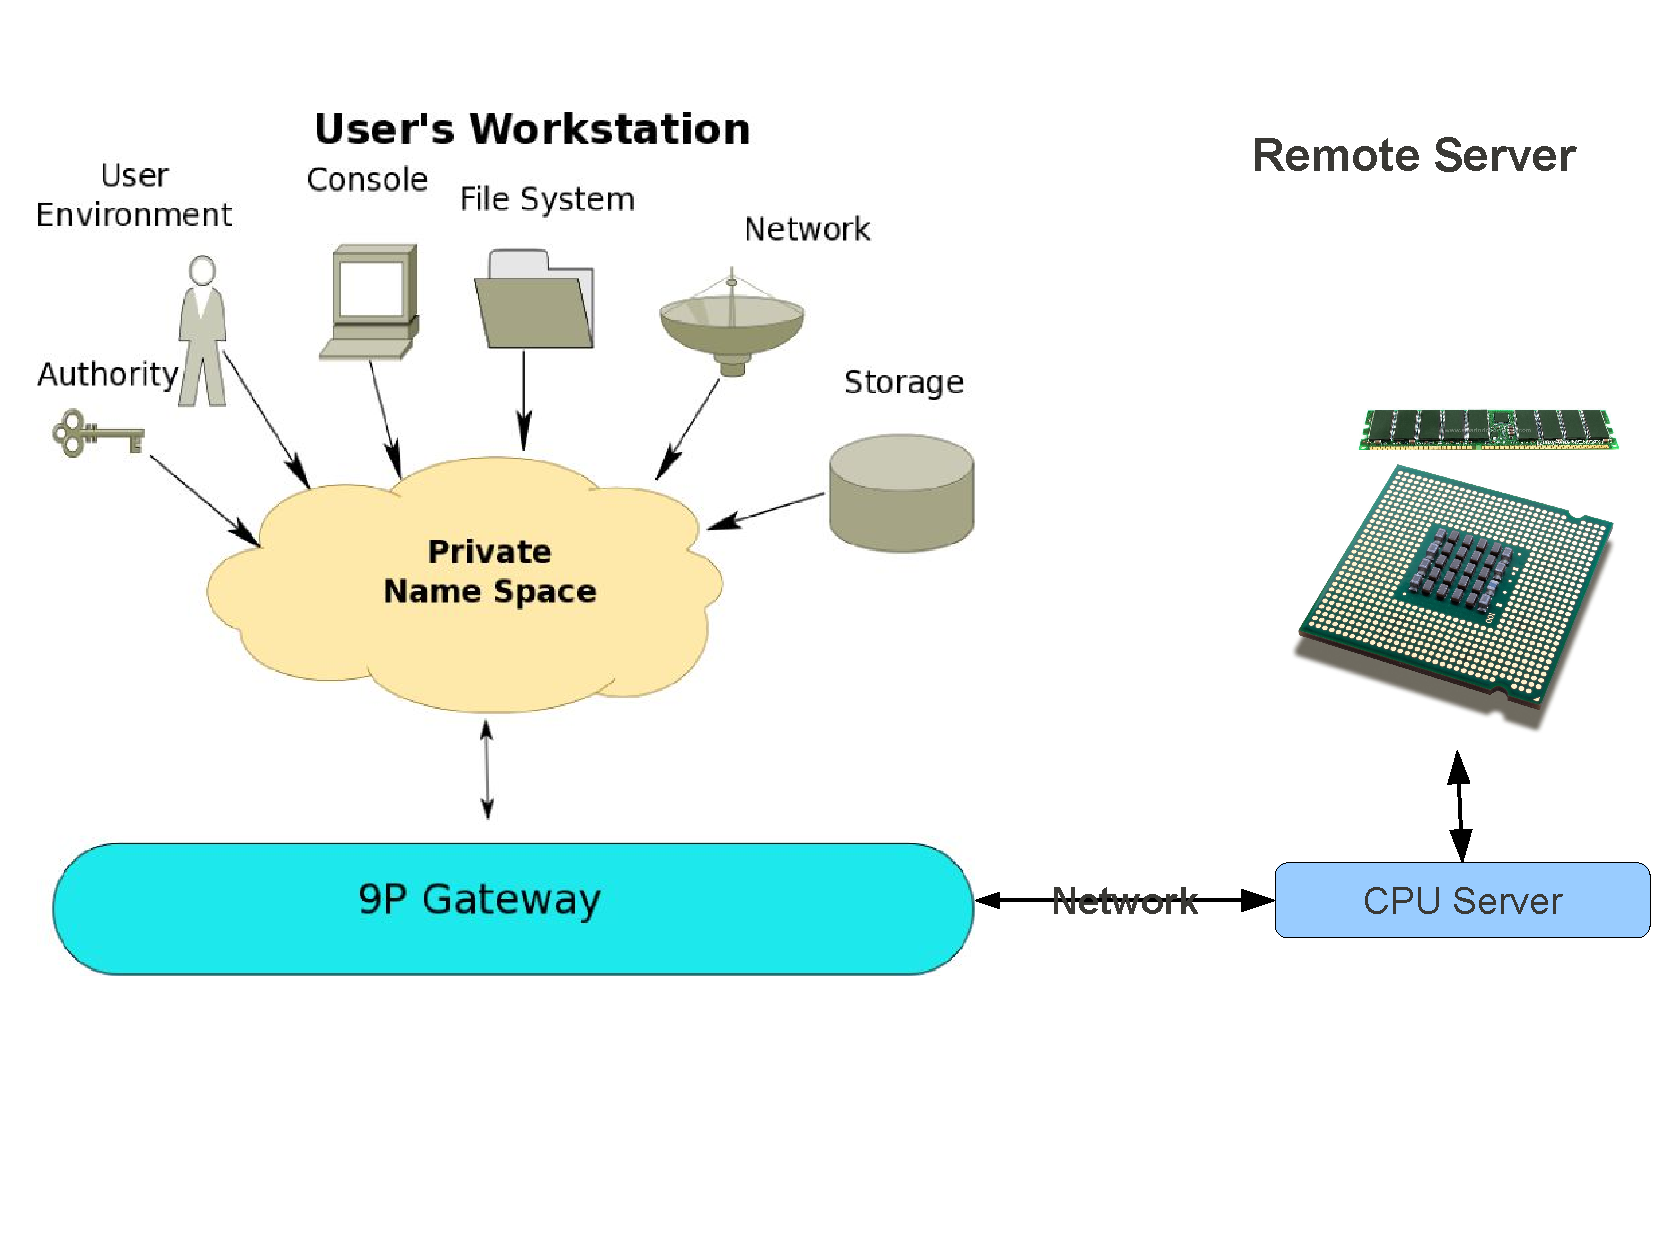
\includegraphics[height=0.4\textheight,width=0.6\textwidth]
		{CPU}
    \fi
    \caption{CPU}
    \label{fig:CPU}
  \end{center}
\end{figure}

It works by creating new private namespace\cite{namespace} with a
local filesystem view, disk, network, console, etc on the client side.  
This namespace is mounted by the remote processor and used for all the processes 
started there as part of the CPU session.  These processes have the view of the client system 
while the execution is still performed on a remote node.  One of the key
advantages of this model is that now users don't have to worry about the environment
of the remote node when running any job on it.  Any execution requested on a remote
node will see the same local view of the user's environment, simplifying the
deployment of applications.

Even though CPU does simplify the life of the developer, it does not solve all of
our problems.  Firstly, it is Plan 9 specific and does not work with any other
operating system.  This keeps it out of realm of most of the users.
Another limitation is that CPU works in one-to-one fashion.  This limits the
usefulness of it in cluster like environments.  Controlling each and every node
in a cluster individually does not scale well for larger numbers of nodes.

\section{XCPU}
XCPU\cite{ron-xcpu} \cite{lucho-xcpu} was an attempt to bring the functionality
of CPU into mainstream operating systems like Linux.  It aims at providing the
remote resources using a \textbf{filesystem interface} and improve the
scalability.  XCPU can be seen as the remote process execution
system presenting execution and control services in the form of files in
a hierarchical filesystem.  This filesystem can be exported over the network so that
other nodes can use it.  As XCPU presents remote compute resources as files,
deployment of applications does not need any special privileges as 
long as user can read/write these files.

XCPU has two types of nodes, the controller node which is responsible for
starting and controlling the job and compute nodes which actually do the computations.

In addition to execution of the program, XCPU is also responsible for 
distributing them to remote nodes. XCPU differs from CPU in that it does not use the 
private namespaces to create local environments on remote nodes.  It uses 
the \textbf{push model} and automatically pushes the executable and all the dependencies 
of it to the remote node.  The dependencies are analyzed using static analysis of 
the executable requested by the user.

To achieve scalable pushing of programs and their dependencies, XCPU uses a few
compute nodes for distributing the programs and dependencies during the program
startup time.  This is known as the \textbf{tree spawn mechanism} and it improves the
scalability for XCPU to larger numbers of nodes.  Figure 2.2 presents a
typical tree hierarchy used by XCPU for better scalability.

\begin{figure}[h]
  \begin{center}
    \leavevmode
    \ifpdf
      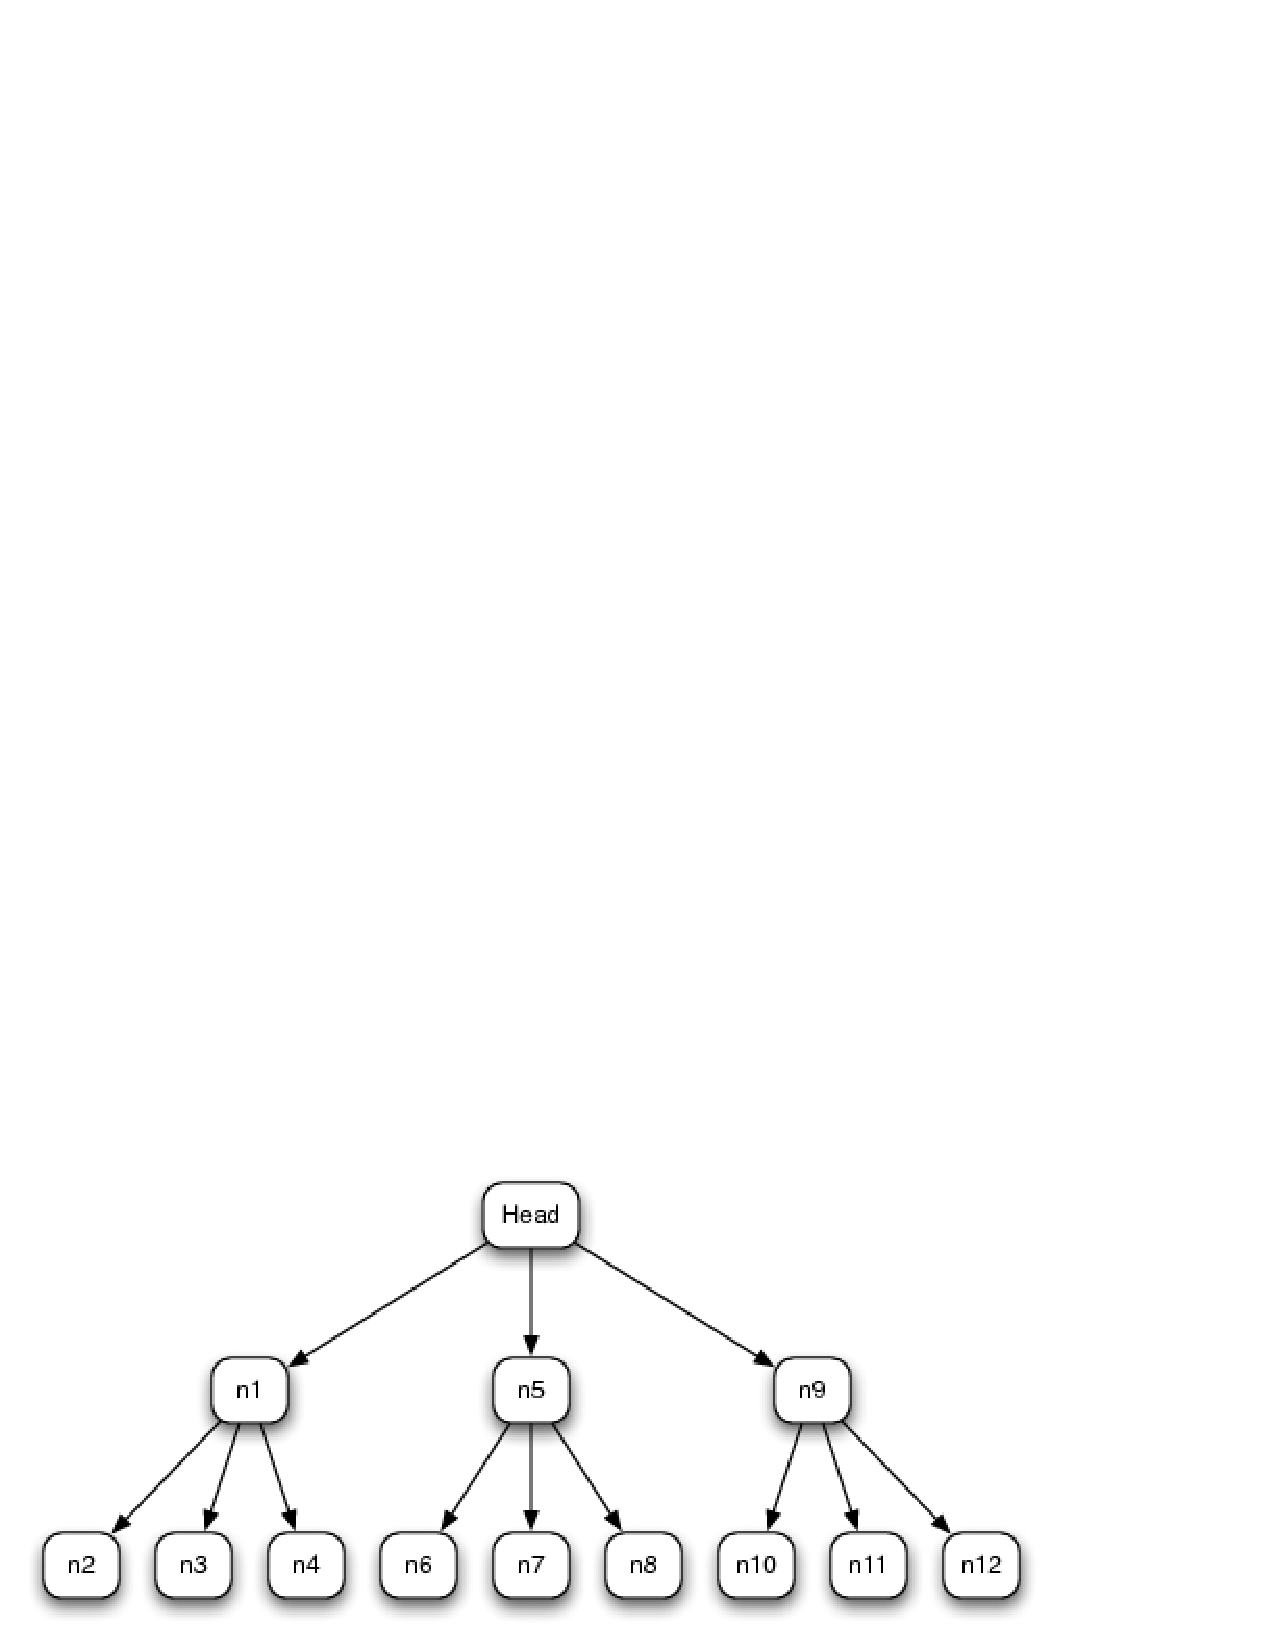
\includegraphics[height=0.3\textheight,width=0.6\textwidth]
		{xcpu-tspawn}
    \fi
    \caption{XCPU tree spawn mechanism}
    \label{fig:XCPU}
  \end{center}
\end{figure}

With automatic pushing and the tree spawn mechanism, XCPU not only simplifies the deployment
of applications but it also scales them better with quicker job startup time.


\subsection{Drawbacks}
One major drawback of XCPU is the result of the push model.  All
dependencies are needed to be pushed to compute nodes.  The difficulty lies
in detecting the dependencies of the requested executable.  Static analysis is
not capable of detecting dependencies like configuration files which are known
only at runtime.  The user needs to explicitly provide information about these
dependencies so that XCPU can push them.


XCPU is designed for executing one application on the cluster at one time.
This is not very useful when multiple users want to use different parts
of the cluster at the same time.  XCPU does not aim for such situations, leading
to limited flexibility.


XCPU has properties like quick job startup time and a simple filesystem
interface which makes it a good first step towards scalable dataflow application
deployment.  But there is still a lot of gap to cover for meeting all the requirements
of dataflow applications.


\section{XCPU2}
XCPU2 \cite{lucho-xcpu2} is evolved from XCPU and is aimed to provide more flexibility.  
XCPU2 was inspired by the use of \textbf{private namespace} of CPU.  Recently the Linux kernel 
has added support for private namespace\cite{linuxns}, and this facilitated the
development
of XCPU2.  The much needed flexibility is provided by the ability of building a separate
view of the filesystem for each process using these private namespaces.

XCPU2 works by dividing the nodes into three categories.  Each type is responsible
for different functionality.
\begin{enumerate}
	\item \textbf{A Control Node} is responsible for handling \textbf{reservation} requests for compute nodes.
There will  be a single control node per cluster for this role.  XCPU2 
does not take responsibility of reservation.  This part is typically delegated
to some other software which accepts the reservation requests and returns the
list of nodes assigned for reservation request.

	\item \textbf{A Job Control Node} is responsible for \textbf{managing a single job}.
The nodes provided by the control node for reservation requests are then managed by 
a job control node which is responsible for starting, stopping the job and manipulating
the filesystem view of compute nodes.  Users will typically interact with these
job control nodes for running their applications.

	\item \textbf{A Compute Node} is responsible for \textbf{actual computation}.
These nodes communicate with the job control nodes and accepts the application names
that are to be executed.  These nodes also allow job control node to modify the
filesystem view of process executing the application by using private namespaces.

\end{enumerate}

A user typically starts by requesting the reservation with the control node.  Once the
reservation is done, the user will get an access to the job control node which can be used
to manage the job.  The user can export his local filesystem view to the job control node
with the name of the executable to execute.  All compute nodes mount the user's local
filesystem via the job control node.  All compute nodes then create processes with
the namespace modified in such a way that it will inherit the user's filesystem view
instead of the compute node's filesystem view.  This way, processes running on a compute node
will see the same uniform view as processes in the user environment.  In contrast to
XCPU which pushes the executables and dependencies, XCPU2 uses the \textbf{pull model}
where any dependency is automatically pulled because of the inherited user filesystem
view using private namespace.

This propagation of the user's environment on the compute nodes simplifies the application
deployment to a great extent.  If an application is properly running on the user environment, then
it will also run on the compute nodes as they have the same filesystem view.  This is
a big improvement over other environments where developers are forced to develop
the applications for an environment of the compute nodes which may differ significantly 
from the user environment.  Also, developers can use any libraries or customized tools 
within a distributed application without worrying much about availability of those
in the compute environment.  Users neither need special privileges nor do they need to make
special requests for installing special libraries and modified tools on every nodes
of the cluster.  This model also simplifies the maintenance of the cluster as there is
no need to maintain every tool and every version of the libraries on each compute node.

\begin{figure}[h]
  \begin{center}
    \leavevmode
    \ifpdf
      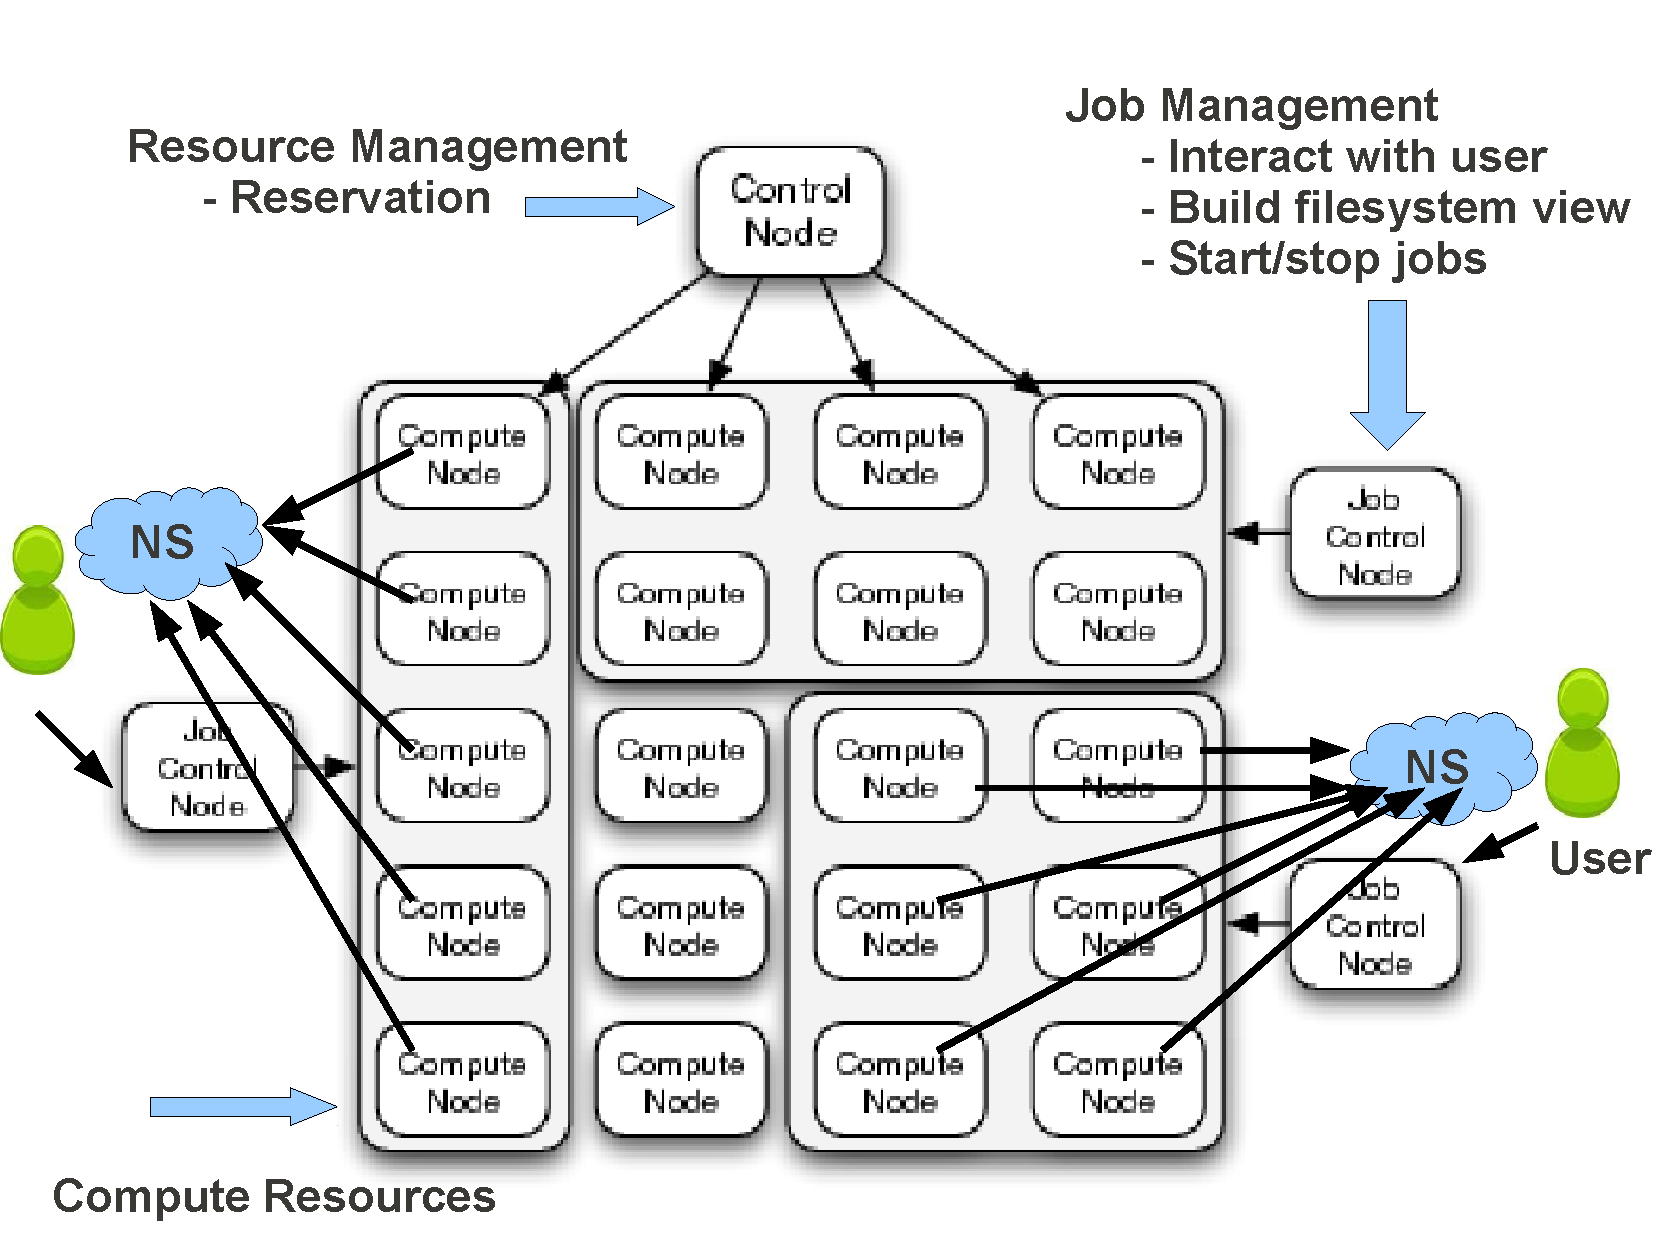
\includegraphics[height=0.3\textheight,width=0.6\textwidth]
		{xcpu2}
    \fi
    \caption{XCPU2 in action}
    \label{fig:XCPU2}
  \end{center}
\end{figure}

The diagram 2.3 shows how multiple users can use the cluster at the same time for executing
different applications with contradicting requirements on the filesystem view.  The control node
provides the partitioned set of compute nodes with one job control node to each
user requested reservation.  Now each user can execute its own application
with  it's own view of filesystem without any interference from other users who
are running their applications at the same time on the same cluster.  This provides added
flexibility and better utilization of resources.

XCPU2 also inherits scalability from XCPU by using the tree spawning mechanism in compute
nodes within a single reservation.  This hierarchical structure reduces the load
on the job control node and provides better job-startup time. 

XCPU2 is definitely a forward step toward providing the flexibility needed to deploy
dataflow applications.  It provides flexibility in controlling the namespace view 
and it allows multiple users to run their applications simultaneously with good
job startup time.

\subsection{drawbacks}

The fundamental drawback with XCPU2 is the granularity of control.
The control provided by the XCPU2 on the filesystem view of compute nodes is not fine
grained.  Users can control the filesystem view of all nodes together, but they
can not control each and every compute node individually.

This lack of control on every node is a major deterrent for dataflow applications.
As these applications can be best scheduled by treating them as DAG and mapping
each computational vertex to one compute node.  As each computational vertex can
have different requirements about environment and filesystem view, control of
each compute node is important for successfully mapping dataflow application
on compute resources.  \textit{XCPU2 fails to provide this much needed fine grained control
on all nodes}.

This limitation was major motivation for us to develop XCPU3 which can handle
all needs of dataflow applications.

% ------------------------------------------------------------------------
%%% Local Variables: 
%%% mode: latex
%%% TeX-master: "../thesis"
%%% End: 
